\documentclass[runningheads,a4paper]{llncs}
\usepackage{amssymb}
\setcounter{tocdepth}{3}
\usepackage{graphicx}
\usepackage{subfig}
\usepackage{algorithmic}
\usepackage{algorithm}

\usepackage{url}
%\urldef{\mailsa}\path|{andersonp,yongkiy,sowmya, bernhardh}@cse.unsw.edu.au|  
\newcommand{\keywords}[1]{\par\addvspace\baselineskip
\noindent\keywordname\enspace\ignorespaces#1}

\begin{document}

\mainmatter

\title{RoboCup Local Game Management System}

%\titlerunning{Game Management System}

\author{Sean Harris  \and Belinda Teh \and \\
    Youssef Hunter \and Richard Hua \and \\
    Bernhard Hengst}

\authorrunning{Sean Harris, Belinda Teh, Youssef Hunter, Richard Hua, Bernhard Hengst}

\institute{School of Computer Science and Engineering,\\
University of New South Wales, UNSW Sydney 2052 Australia}

%\toctitle{Game Management System}
%\tocauthor{Sean Harris}
\maketitle


\begin{abstract}
Refereeing a soccer game is no easy feat for a human as decisions made under pressure are prone to mistakes and subjectivity. Spectating a RoboCup match is not particularly rewarding either, especially when game progress is hard to follow and there are large crowds surrounding the fields. As such, this research aims to create robot referees to assist human referees, as well as to create a large visual and meaningful display of RoboCup games. By building on existing infrastructure on the Aldebaran Naos for ease and code reuse, a robot referee system consisting of four Naos placed strategically around the field was successfully prototyped for the Standard Platform League. They were able to filter and track the ball and robots as a team, and detect if the ball had gone out or into a goal. This information was then translated into vocal and physical announcements by the robot referees, as well as into a meaningful display of the field. The robots were also able to display their view of the game depending on whichever was closest to the ball, and communicate with the game controller to show the current score. Though many features remain to be implemented, such as audio commentary or video replays, there is much potential for robot referees to improve the RoboCup experience for both human referees and the wider audience.
\end{abstract}


\section{Introduction}

Refereeing any sport is a very challenging exercise and referees are often subject to a great deal of pressure and criticism.
During games, mistakes can be made, whether they be due to a lack of information, a varied interpretation of the rules, or even just a difficult situation.
These problems are highlighted at RoboCup where referees are often new and inexperienced.
Refereeing games is also a difficult task as there are often a large number of simultaneous events that all require attention.
Having an automated refereeing system to aid referees would alleviate much of this pressure, as well as remove the human error and subjective element to many refereeing decisions.

Another issue highlighted at RoboCup is that the games do not provide a high quality spectator sport.
This is partially due to the lack of infrastructure aimed at providing game state information to the crowd.
At present, the audience stand in a clump around the field fighting for a good view of the action, with many not actually understanding what is happening.
With an automated audience display, large TVs could be positioned around alternate seating locations for people to experience the live broadcast comfortably.

The following sections outline the innovations undertaken to produce such a system. Namely, these improvements cover:
\begin{itemize}
\item Audio and visual relaying of the ball's in/out and goal status to the referee and audience
\item Automated camera switching and streaming
\item Increase in ball position accuracy through the use of combined data from individual Extended Kalman Filters
\item Perspective geometry using fields lines to further increase ball position accuracy
\item Robot player location saliency through the use of a grid filter
\end{itemize}

\section{Background}

In 2008, the University of Chile proposed the use of a separate service robot as a referee for the Humanoid League.\cite{Arenas2009}
It would move along one side of the field, using its own camera to analyse game actions at up to 20 FPS, communicate to humans via speech, and to robot players over wireless.
However, this system was trained on detecting Humanoid League defined features only, not to mention that its movement would result in less accurate localisation and its wireless communication could interfere with team messages during gameplay.
The system also did not encompass any sort of visual display for catering to large crowds and noisy environments.

When SPL was still based on the Sony Aibos, Carnegie Mellon University prototyped a team of two humanoid game commentators which stood on the sidelines of the field.\cite{veloso2008}
Using input from their vision, the game controller, and human intervention, they were able to translate events into a set of predefined announcements.
However, this too had to be built separate to the existing soccer system, and had no appropriate spectator display.

The Game Controller allows referees to send messages to the robots for events such as a goal or a penalty.
While it provides an overview of the game state to the referee, such as the score, time remaining and robot status, it does not provide any information regarding the location of the ball or robots, and requires manual input for most game state changes.
The Game State Visualiser is a program that reads from the Game Controller in order to display the current score to the audience.
These programs, while useful, provide an extremely limited amount of information to the audience and are not substitutes to actually watching the game.

Our construction of a robotic referee system thus aims to deal with these issues. Namely, by reusing the systems built for the Naos in the Standard Platform League which already tackle the similar problems of localisation and tracking in robot refereeing. By giving each referee a set and still position, we can take advantage of the reduced noise and combine information from each robot referee to further improve game data such as ball and robot locations. With the modification of existing debugging and visualising tools, this data can be translated to a meaningful visual and audio display for the audience.

\section{Audience Engagement}

The main component of the game state display is the bird's eye field view on the left, which shows the current location of the ball and robots as perceived by the robot referees.
The blue team's score is shown on the bottom left whilst the red team's score is shown in the bottom right.
Status messages for the ball such as `Out' and `Goal' (in their respective colours) would also be displayed in the centre.

\begin{figure}[h!]
  \centering
  \subfloat[Out]{\label{fig:display-out}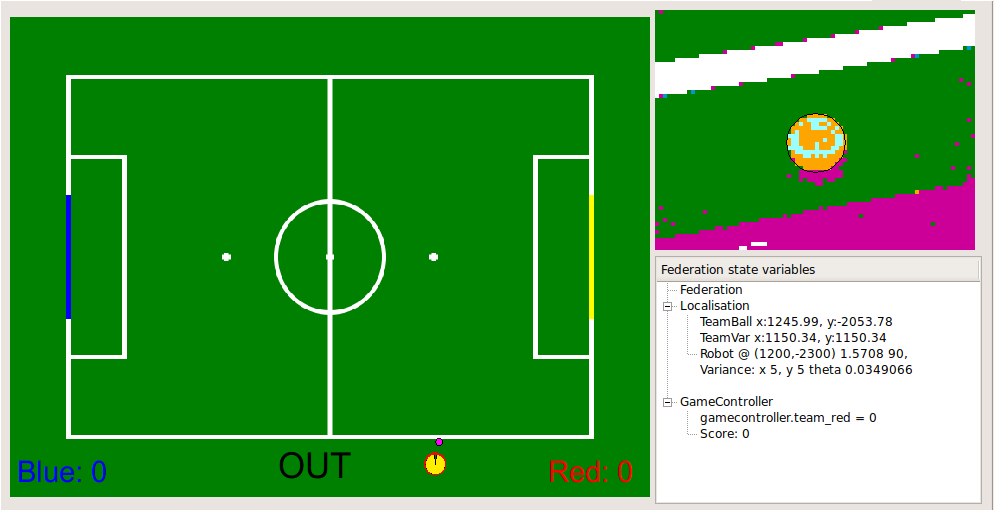
\includegraphics[width=0.6\textwidth]{figures/display-out}}
  \subfloat[Goal to Blue]{\label{fig:display-goal}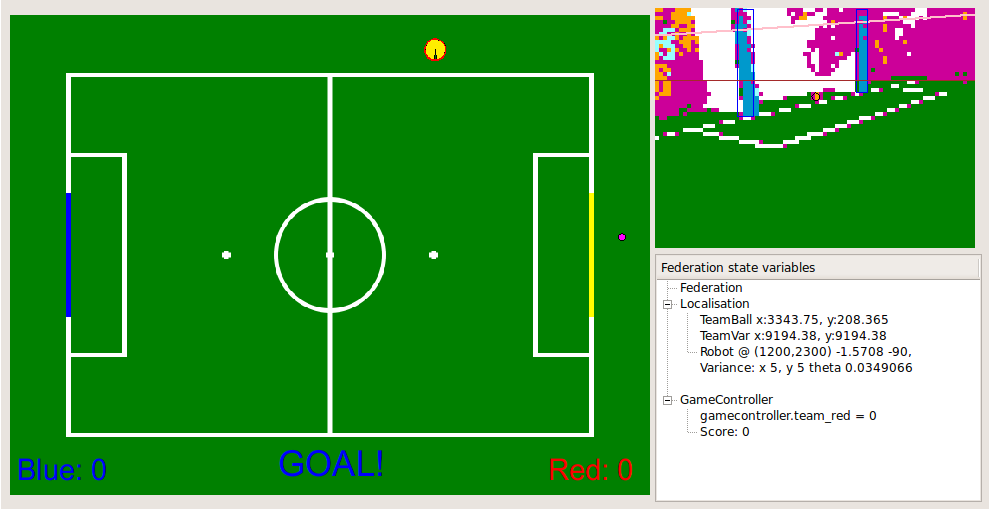
\includegraphics[width=0.6\textwidth]{figures/display-goal}}
  \caption{Varying instances of the game state display\label{display}}
\end{figure}

If the robot referees detected that the ball had gone out or into a goal, they would announce `Out', `Goal blue' or `Goal red' in order to notify both the human referees and the audience.
Upon scoring a goal, the referees would also raise their left or right arms to signify the direction in which it had been scored. 
On any score update received from the Game Controller, another vocal announcement would be made for the benefit of the spectators.

In the top right section, actual camera footage is streamed from which ever referee has the best view of the ball, and could be switched around if the ball moved across the field or became obstructed by players.
The robot with the best view is decided by its proximity to the ball as well as the time since it had last seen the ball (see Algorithm 1).

\begin{algorithm}
\caption{Camera Switching Algorithm}
\begin{algorithmic}

\STATE $best \leftarrow max$
\FORALL {$robots$}
  \STATE $distance \leftarrow \sqrt{(ball.x - position.x)^2 + (ball.y - positions.y)^2}$
    \IF{$distance < best - j \AND ballLostCount < k$}
        \STATE $best \leftarrow distance$
          \ENDIF
          \ENDFOR

\end{algorithmic}
\end{algorithm}

To emulate the circumstances of a real game, two opposing robots were placed on to the field to test the camera stream from all four referee robots.
There were several instances where the ball was lost due to obstruction, particularly when robots clumped around the goals.
However, since the stream would be left with the last robot with the best view, regaining sight of the ball once the occlusion had moved was rather trivial.
Often one of the further robots with a better angle would still be able to see the ball, and could thus step in to stream the game.

The robot referees interaction with the audience was received rather well, especially in the ways they emulated human soccer referees upon announcing a goal.
Camera switching and streaming between the referees was quite a success as they were able to consistently provide a view of the action.
The only issue some audience members had was when the ball rolled through the middle of the field and in range of three of the robots.
It would cause the stream to switch quickly between all three, resulting in a rather disorienting effect.
However, this could easily be solved by adding a timer between switches to slow the process down enough for the human eye.


\section{Ball Tracking}
Having accurate knowledge of the position of the ball during play is obviously a crucial element to any potentially effective refereeing system. At the simplest and most important level, the position of the ball determines rulings regarding goal scoring and out of bounds. The position of the ball also provides a central focus of spectator attention - with the most interesting moments of the game almost always revolving around the ball's position and the robots interacting with it.

Humanoid Nao robots serve as the platform for the referee system, observing the game from their stationary positions around the edge of the field. As the Nao is also the standard platform of the SPL, using them as the referees allows for the reuse of many of the systems and tools that were developed for the actual players. An Extended Kalman Filter (EKF)\cite{kalmanintro} was developed to use the inherently noisy vision information from the observing referee Naos to track the position of the ball as the players and play progress about the field.

The hard-coded stationary positions of the referee robots ensure that localisation noise does not interfere with the tracking of the ball through vision observations. These observations are received as polar coordinates, with the observed ball being represented as a certain distance (r) away from the robot, and at a certain heading ($\theta$). Of significance in our approach is to incorporate an assumption that the uncertainty of the observation's distance and heading is not equal: it is assumed that the observation's heading coordinate is more reliable than the distance. Essentially, when processing observations of the ball, more confidence can be placed in the perceived direction of the ball relative to the robot, over its perceived distance from the robot.

This assumption is reflected in the variances associated with the components of the polar observations when passed to the EKF. The variance of the observation's heading is kept constant, while the variance of the distance is calculated as a function of the perceived distance itself; with the variance of the distance increasing the further away the ball appears to be. The EKF that was developed takes the polar observation coordinates and their variances as input, but uses the observation Jacobian matrix below to transform the coordinates into Cartesian form, and track the ball using an absolute positioning scheme.

\[
H = 
\left[ \begin{array}{cc}
\frac{\delta r}{\delta x}        &       \frac{\delta r}{\delta y}         \\
\frac{\delta \theta}{\delta x}   &       \frac{\delta \theta}{\delta y}    \end{array} \right]
=
\left[ \begin{array}{cc}
\frac{x}{\sqrt(x^2 + y^2)}        &       \frac{y}{\sqrt(x^2 + y^2)}         \\
\frac{x}{x^2 + y^2}   &       \frac{y}{x^2 + y^2}    \end{array} \right]
\] 

The filter also transforms the variances of the distance and heading, and calculates a covariance matrix for the Cartesian coordinates of the ball estimate. This covariance matrix can then be used to display a visual representation of the uncertainty of the filter's ball estimate; an ellipse is expected to reflect the higher variance of the distance component. 

To improve the coverage of the playing field and the accuracy of ball tracking, four referee robots are used, each placed in a hard-coded position a short distance from the field edge (visible in Figure \ref{fig:referees}). These four referees are each capable of observing the ball and making their own estimates complete with an elliptical covariance. As each referee observes the field from a different angle, these ellipses can easily be combined to effectively provide a more accurate estimate of the ball's position. The weighted mean of each of the referee's estimates is calculated to become the team's estimate (also with an accompanying covariance matrix). Figure \ref{fig:combination} shows a rough example of how these individual variance ellipses can combine. 

\begin{figure}
  \centering
  \subfloat[Referee Naos]{\label{fig:referees}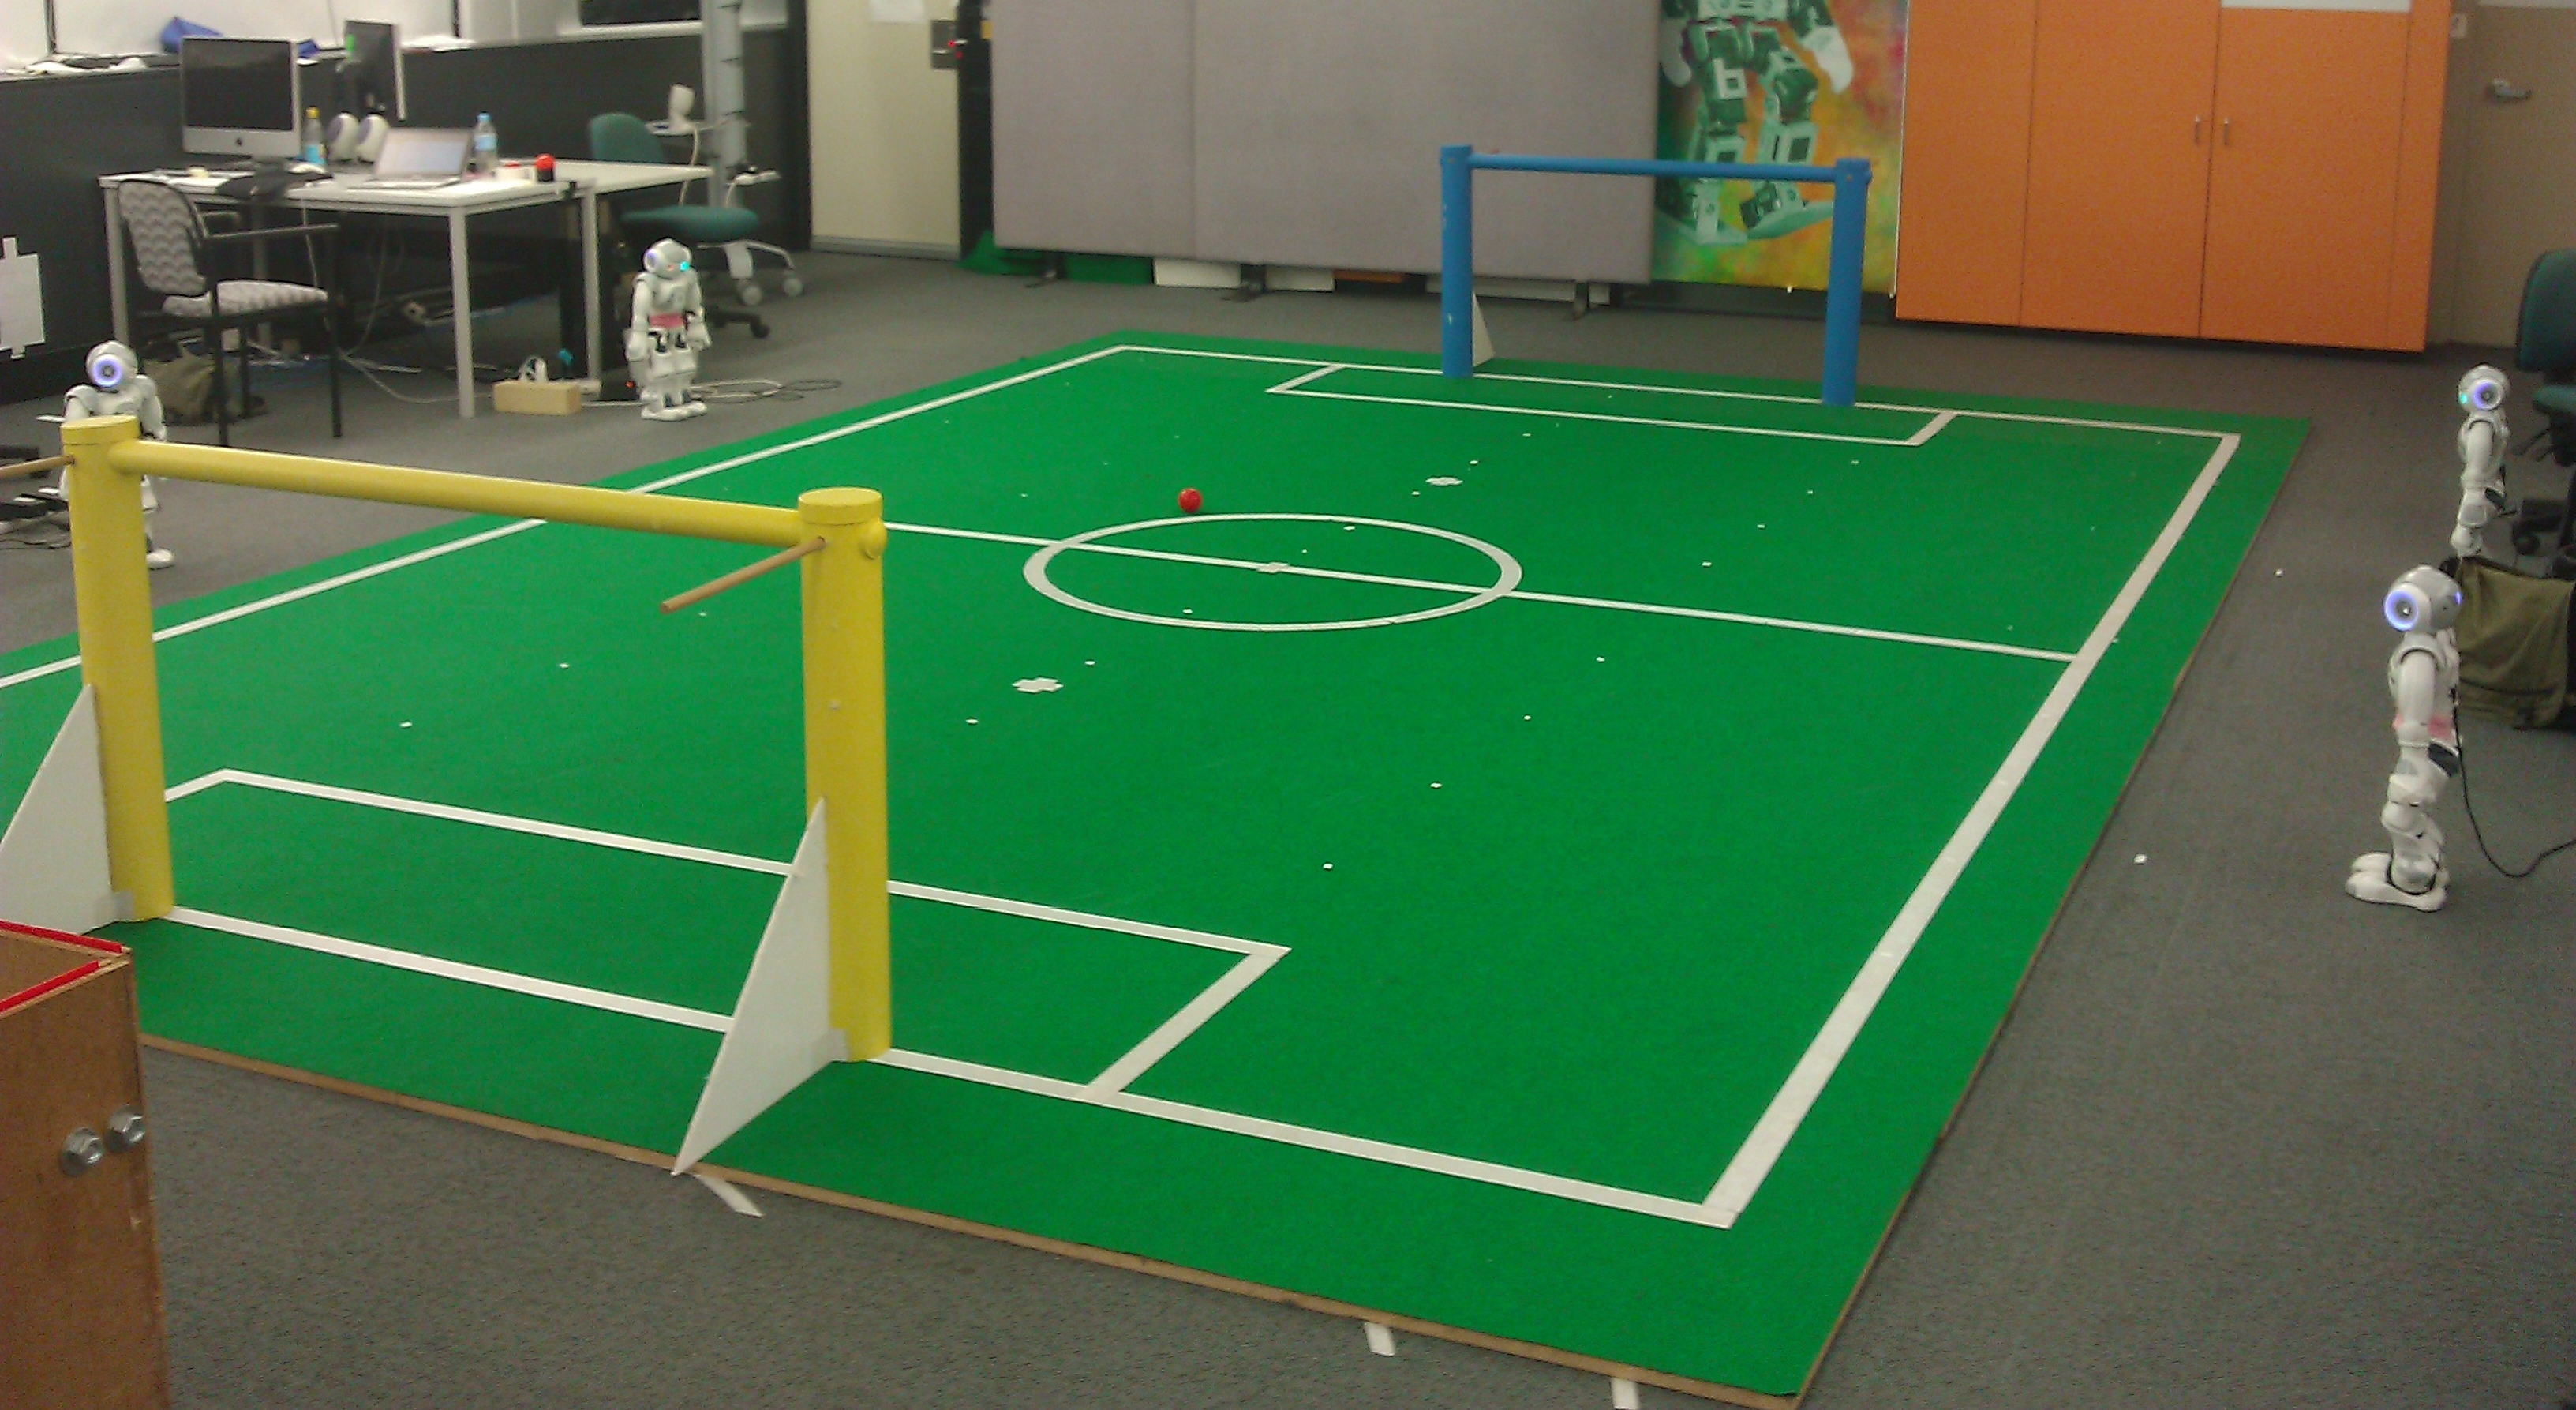
\includegraphics[width=0.675\textwidth]{figures/referees2}}~                
  \subfloat[Ellipse Combination]{\label{fig:combination}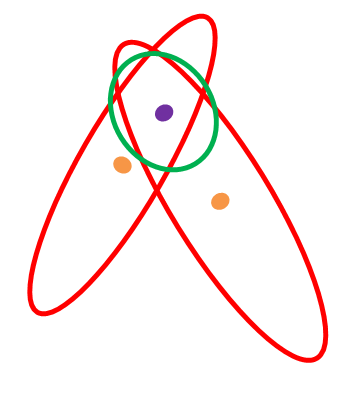
\includegraphics[width=0.325\textwidth]{figures/example}}~
  \caption{Referees observe from their positions and combine their infromation}
  \label{fig:TeamUpdates}
\end{figure}

The team's estimate of the ball also serves another purpose; if a robot referee cannot observe the ball directly, but the team as a whole is aware of the ball's position with a high enough degree of certainty, then the robot will look in the direction that the team perceives the ball to be. In this way, a robot can track the position of the ball without personally observing it - allowing it to be ready to observe the ball as soon as it approaches or becomes less obscured, or to still provide the closest video feed to the audience.

\begin{figure}[h!]
  \centering
  \subfloat[Sideline]{\label{fig:sideline}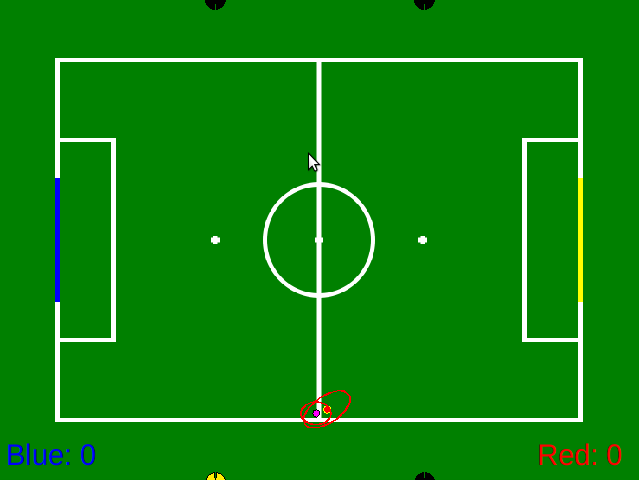
\includegraphics[width=0.5\textwidth]{figures/ellipse-sideline}}  
  \subfloat[Goal Box]{\label{fig:goalbox}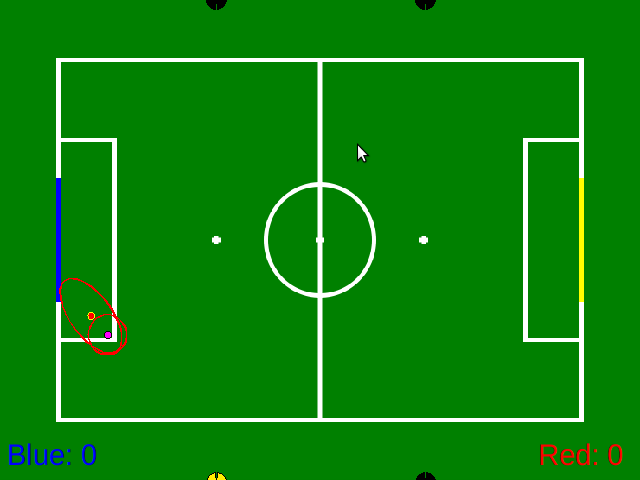
\includegraphics[width=0.5\textwidth]{figures/ellipse-goalbox}}
  \\
  \subfloat[Centre]{\label{fig:centre}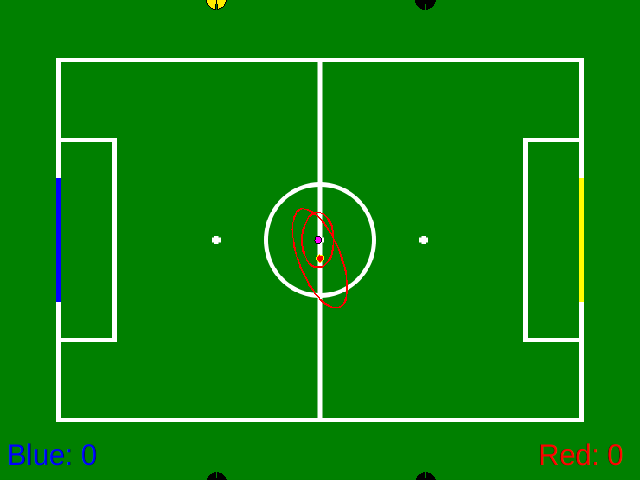
\includegraphics[width=0.5\textwidth]{figures/ellipse-centre}}
  \caption{Individual and Team Ball Estimates\label{ellipse}}
\end{figure}

In Figure \ref{ellipse}, the yellow half-circle on the edge of the screenshots represents the referee that is serving as the reference robot; whose filtered estimate of the ball is represented by the red dot with yellow outline at the centre of its elliptical covariance. The purple dot with its more spherical covariance represents the combined team ball estimate.

From the screenshots, it can be seen that the elliptical covariance of the individual estimate in each of the three cases changes in both angle and magnitude, depending on the direction and distance of the observed ball. The table below provides a quantitative (mm) summary of the three scenarios pictured; comparing the reference robot's individual filtered estimate, with the combined team ball estimate and the actual position of the ball. It is clear that the combined team ball provides a more correct estimate of the ball's position, and the team ball covariance ellipses visible in the screenshots indicates that by combining the estimates of the individual referees, the resulting team estimate is a less uncertain hypothesis.

\begin{figure}[H]
\begin{center}
    \begin{tabular}{ | l | l || l | l || l | l | }
    \hline
    \multicolumn{2}{|c||}{Actual Position} & \multicolumn{2}{|c||}{Individual} & \multicolumn{2}{|c|}{Team} \\ \hline
    \multicolumn{1}{|c|}{Place} & \multicolumn{1}{|c||}{Coordinates} & \multicolumn{1}{|c|}{Estimate} & \multicolumn{1}{|c||}{Error} & \multicolumn{1}{|c|}{Estimate} & \multicolumn{1}{|c|}{Error} \\ \hline
    Sideline & (0,-2000) & (81.0, -1880.1) & 144.7	& (-41.3, -1924.5) & 86.1 \\ \hline
    Goal Box & (-2400,-1100) & (-2638.8, -836.3) & 355.8 & (-2447.9, -1047.3) & 71.2 \\ \hline
    Centre & (0,0) & (-12.4, -195.6) & 196.0 & (-32.6, 5.7) & 33.1 \\ \hline
    \end{tabular}
\end{center}
  \caption{Table showing the improvement in ball tracking}
 \label{fig:ballpos}
\end{figure}


The Extended Kalman Filter that was developed for the referee system used assumptions regarding distance and heading variances to compute individual estimates for each robot, and this assumption is successfully reflected in the covariance ellipses visible in the results. These individual estimates are also successfully combined to produce a more accurate, correct, and reliable team ball estimate. Overall, this system proved to be quite successful in achieving its goal of an accurate and robust ball tracking system.


\section{Field Line Updates}

As described earlier, a big focus of this project is determining whether the ball is in or out. The decision as to whether the ball is in or out is defined in the rules relative to the field line, so it makes sense to utilise relative distances to make this decision rather than simply relying on the Kalman Filter. Thus a new EKF update utilising nearby field lines has been developed. The premise is to use the relative distance between the ball and a nearby field line to update the position of the ball. This field line can be matched to a global map of the field and the relative distance to the ball can be utilised to determine the ball's global position on the field. 

\begin{figure}[h!]
  \centering
    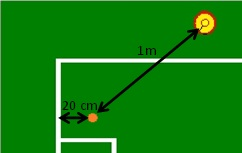
\includegraphics[width=0.5\textwidth]{figures/BallDemo.jpg}
  \caption{The ball is much closer to the field line than the robot}
 \label{fig:balldemo}
\end{figure}

Figure \ref{fig:balldemo} shows how when the ball is near the goal box, the distance from the ball to nearby field lines is far shorter than the distance to the robot. Using the traditional Kalman Filter method, the position of the ball becomes less accurate as it gets further away. With this new update however, the ball position becomes more accurate as we get closer to the line because the relative distance from the ball to the line is becoming smaller. This allows for a huge increase in accuracy at the most important location on the field, near the side lines and goal lines.

The first step in this process is to identify the ball and all the nearby field lines. Chatfield's\cite{chatfield} Ball Detection algorithm uses a high resolution fovea to find the ball in each image. Harris's\cite{harris} Field Line Detection algorithm examines both the high resolution ball fovea and a low resolution 80x60 saliency image for nearby lines and stores them in a list.

The list of lines generated above then needs to be matched to actual lines on the field. This involves translating the field lines into global field coordinates by taking into account the current position of the robot. The lines are then matched using distance and direction to actual lines on the field. The ball is also translated into global coordinates in a similar fashion.

The next step is to determine the relative distance from the ball to each line. This is a simple calculation using the distance from a point to a line and is repeated once for each line in the image. The global position of the ball is then updated to reflect its distance from the line, before being converted back to robot relative coordinates and passed into the EKF.

The result of each update is that we have a fairly low variance in either the x or y direction (globally) and a high variance in the other. The combination of this update with the elliptical covariances described above, or even with perpendicular lines, can result in an extremely accurate ball detection with a very low variance. The images in Figure \ref{fig:flellipses} show the improved ball position and reduced variance with this new update running.

\begin{figure}[h!]
  \centering
  \subfloat[Sideline]{\label{fig:flsideline}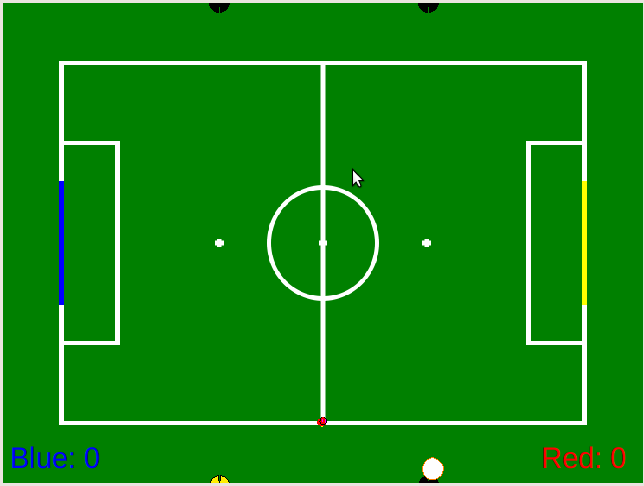
\includegraphics[width=0.5\textwidth]{figures/fl-sideline}}
  \subfloat[Goal Box]{\label{fig:flgoalbox}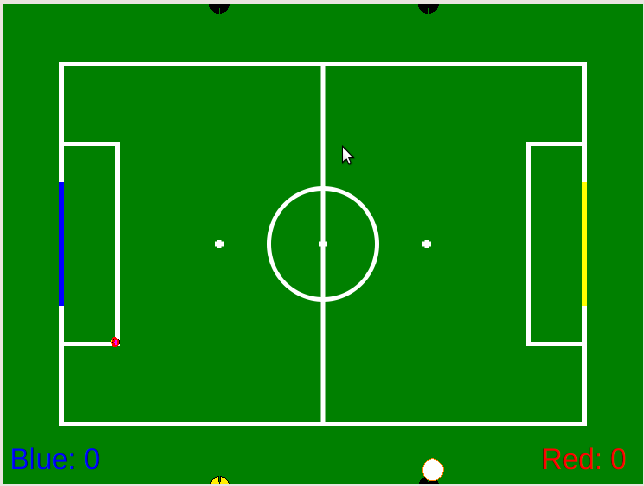
\includegraphics[width=0.5\textwidth]{figures/fl-goalbox}}
  \\
  \subfloat[Centre]{\label{fig:flcentre}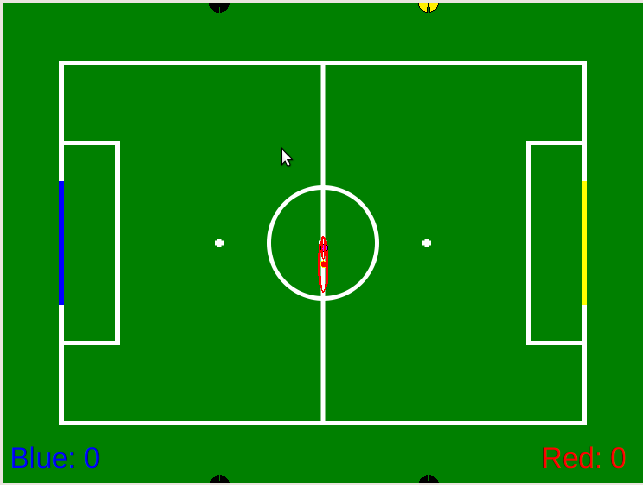
\includegraphics[width=0.5\textwidth]{figures/fl-centre}}
  \caption{Individual and Team Ball Estimates using nearby field lines\label{fieldlines}}
  \label{fig:flellipses}
\end{figure}

The addition of the nearby field line update improved the accuracy of the ball location near lines by a significant factor. Not only was the ball position from each individual robot more accurate and more certain, but the combined team ball position was also more accurate and more certain than before. Table \ref{fig:flballtable} shows the accuracy of the ball across a small number of positions on the field. This result is a significant improvement, especially when compared with the results in Table \ref{fig:ballpos}.

\begin{figure}[H]
\begin{center}
    \begin{tabular}{ | l | l || l | l || l | l | }
    \hline
    \multicolumn{2}{|c||}{Actual Position} & \multicolumn{2}{|c||}{Individual} & \multicolumn{2}{|c|}{Team} \\ \hline
    \multicolumn{1}{|c|}{Place} & \multicolumn{1}{|c||}{Coordinates} & \multicolumn{1}{|c|}{Estimate} & \multicolumn{1}{|c||}{Error} & \multicolumn{1}{|c|}{Estimate} & \multicolumn{1}{|c|}{Error} \\ \hline
    Sideline & (0,-2000) & (-19.6, -1991.7) & 21.3 & (-8.2, -1975.8) & 25.6 \\ \hline
    Goal Box & (-2400,-1100) & (-2401.5, -1083.3) & 16.8 & (-2385.1, -1086.6) & 20.0 \\ \hline
    Centre & (0,0) & (-5.4, -227.1) & 227.1 & (-1.7, -49.3) & 49.3 \\ \hline
    \end{tabular}
\end{center}
 \caption{Table showing the improvement in ball tracking from the relative field line update}
  \label{fig:flballtable}
\end{figure}

You will notice that the accuracy of the ball near the centre of the field is not improved by the addition of this update. In this sample it is actually slightly worse than the original location, however not by a significant amount. It is worth noting that although the overall position of the ball is not correct, the global x position is extremely accurate due to the field line update.

The greater improvements to accuracy are noticeable in the first two rows, which are locations on the field near more than one field line. It is here that this update is able to provide a huge improvement on the location of the ball as it can get a very strong global x and y update on the ball position. 

As mentioned, detecting if the ball is in or out is vitally important to any game refereeing system. This innovative update allows the system to accurately locate a ball relative to a field line, resulting in a significant improvement in ball in/out detection. 

\section {Robot Tracking}

Our solution to the problem of robot tracking is an implementation of a probabilistic grid filter.\cite{ProbabilisticRobotics} We divide the field into 200mm x 200mm grid squares, and continuously update the probability of a robot occupying each square at each time-step. The likely locations of each robot are hence represented by local maxima, with the height of each peak representing the certainty of each hypothesis.

We implemente the process update using a simple Gaussian blur to account for the potential motion of observed robots in all directions. Taking advantage of a Gaussian's linearly separable property, we convolve a one-dimensional kernel with the grid horizontally and vertically in two separate passes to achieve greater efficiency.

For the observation update, we represent observations using Gaussian probability distributions in (r, $\theta$) space. Again, we use a Gaussian's linearly separable property to generate Gaussians in r and $\theta$ separately for efficiency reasons. Using the assumption that the error in camera angle is a fixed constant, we represented the variance in $\theta$ as a constant and use trigonometry and calculus to derive the variance in r, which increases rapidly with distance.

Because a Gaussian drops toward zero with distance, hence effectively serving as an observation that no robot is present, we merge multiple observations from single robots using the inclusion-exclusion principle to prevent contradictory overlaps. Furthermore, when a robot makes no observations, we use a small constant to represent the observation that no robot is present within the field of view. Before applying our observations, we scale them using an observation model to account for parameters of our vision system, including the rate of false positives and false negatives.

We tested the filter on one half of the field, using two referee robots observing a third robot at nine pre-defined locations. We collected data from 500 time-steps of the filter at each of these locations and collected the average of these results.

\begin{figure}[H]
\begin{center}
    \begin{tabular}{ | l | l | p{3cm} | p{3cm} | }
    \hline
    	Experimental Run & Rate of Observation & Average Observation Error (mm) & Average Filter Error (mm) \\ \hline
	1 & 4\% & 110 & 98 \\ \hline
	2 & 0\% & NA & NA \\ \hline
	3 & 24\% & 150 & 36 \\ \hline
	4 & 30\% & 162 & 182 \\ \hline
	5 & 69\% & 268 & 145 \\ \hline
	6 & 16\% & 108 & 159 \\ \hline
	7 & 43\% & 177 & 149 \\ \hline
	8 & 25\% & 185 & 97 \\ \hline
	9 & 18\% & 125 & 111 \\ \hline
	Average & 25\% & 161 & 122 \\ \hline
    \end{tabular}
\end{center}
  \caption{Table showing the performance of the grid filter.}
 \label{fig:gridexperiment}
\end{figure}

The effectiveness of the filter can be seen in the lower overall error despite wildly differing rates of observation input, demonstrating the impact of the applied observation model. Given the fluctuating rate of observation, future improvements to vision software and hardware can be expected to significantly improve the performance of the filter.

It is worth noting that in Runs 4 and 6 of Figure \ref{fig:gridexperiment}, the error in the position reported by the filter was higher than the average observation error. This discrepancy can be attributed to the fact that the grid filter uses a discrete representation of the world while observations are made in a continuous space, introducing errors due to the `rounding' effect.

The current robot tracking system is still very simple. In future, the grid could be modified to track velocity, providing a much more accurate process update. Furthermore, although the observation update is currently approximated by sampling a continuous Gaussian, other more suitable distributions could be used in future. Perhaps most importantly, a finer grid resolution will serve to improve the accuracy of the filter. These improvements should be computationally feasible given that the processing is done inside the game management system as opposed to on the robots.

\section{Future Work}

Many improvements remain to be made in order to create a fully functional robotic referee system. These include filter adjustments to increase position accuracy such as the addition of velocity tracking to better predict future positioning. In terms of audience engagement, future possibilities include the addition of auto-generated audio commentary, replays of camera streams and additions to the bird's eye display such as time remaining, current half and team names.

\begin{figure}[h!]
  \centering
    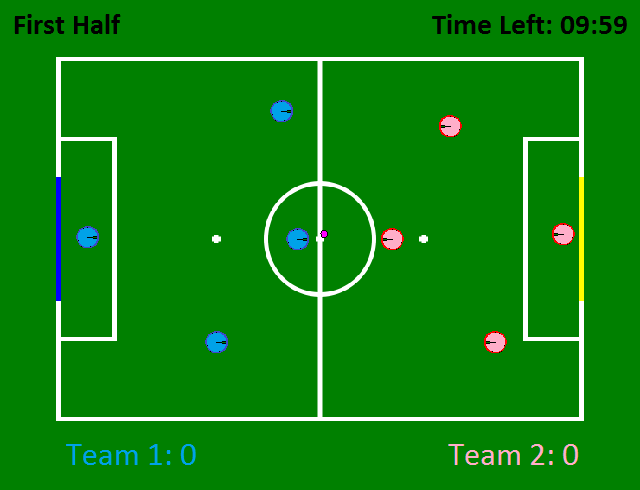
\includegraphics[width=0.6\textwidth]{figures/display-future}
  \caption{Possible future bird's eye display of the field}
\end{figure}

\section{Conclusion}

Accurate ball tracking, camera streaming and robot tracking have benefited audience members with a better and more exciting overview of the game, while even the simple messages of goal and out have helped alert human referees to situations they should be looking out for.
From these preliminary results, it is clear that the refereeing system has a lot to offer RoboCup.
It would allow for more standardised refereeing, reducing the errors caused by inexperienced or pressured referees.
It would also significantly improve the viewing experience of spectators as there would be a lot more game state information available to them, as well as potentially entertaining commentary and replays.

\bibliographystyle{plain}
\bibliography{hengst}

\end{document}
